
\begin{figure}[H]
\centering
\caption{Protótipo Interface Mobile - Tela de Login}
\label{fig:interface-mobile-tela-login}
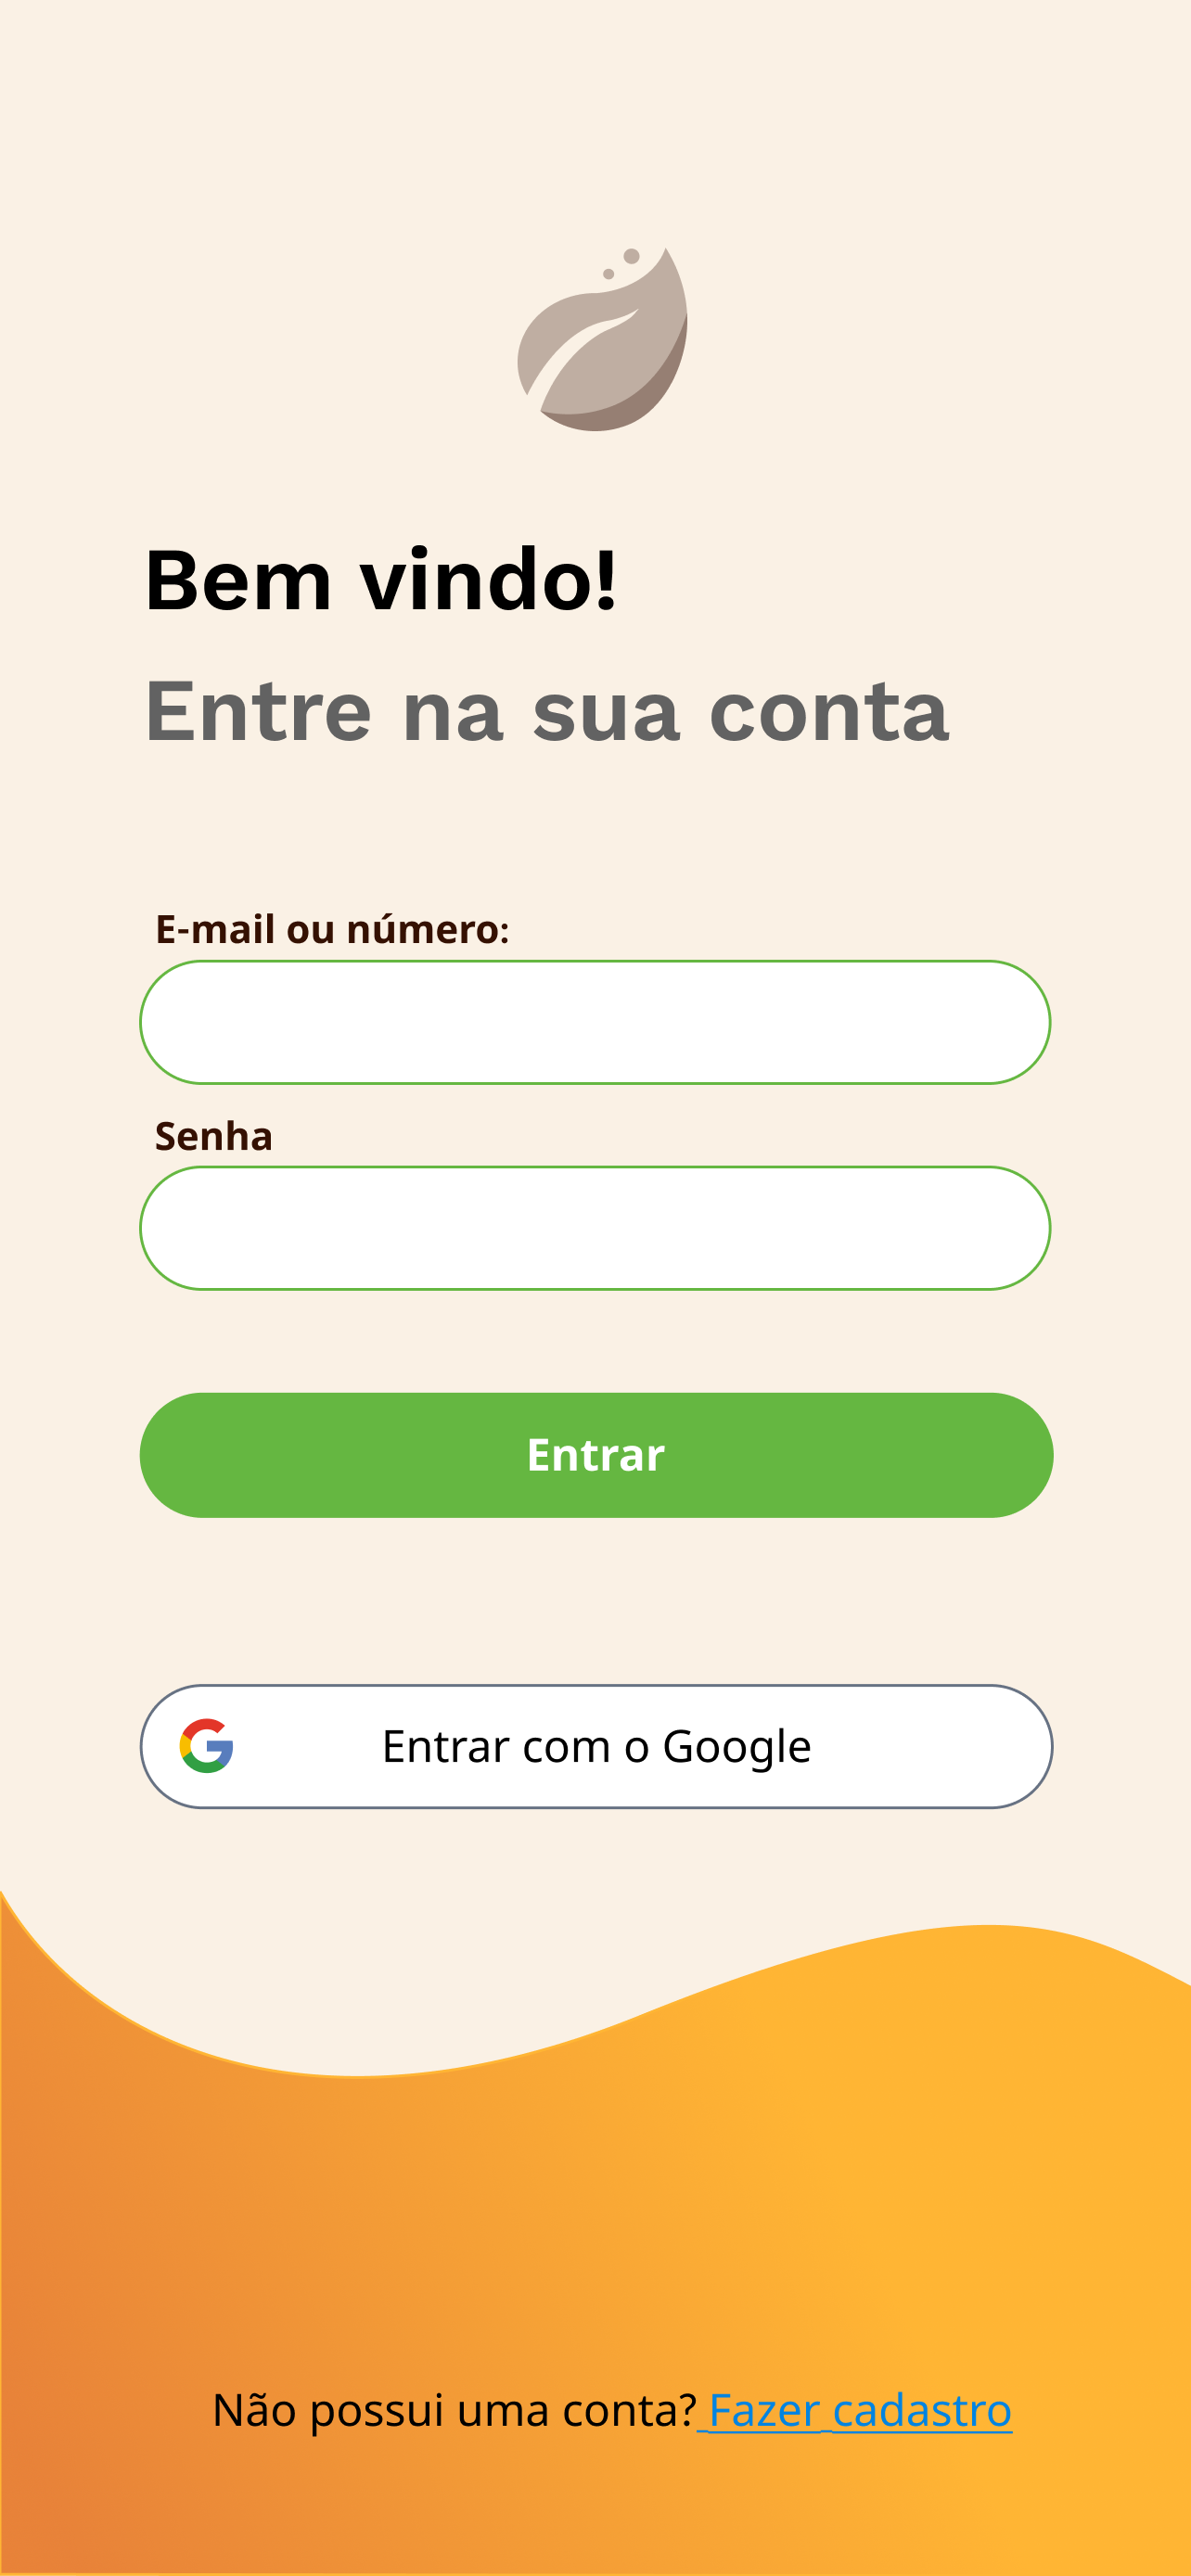
\includegraphics[width=0.2\textwidth]{Images/MobileLogin.png}
\SourceOrNote{Equipe 21 - Vitalliz (2025)}
\end{figure}

A tela de login é o ponto de entrada do sistema. A versão mobile mantem a
funcionalidade e visual da versão web, adaptada para ficar mais agradavel no uso 
de dispositivos móveis.
\medskip


\begin{figure}[H]
\centering
\caption{Protótipo Interface Web - Tela de Início}
\label{fig:interface-web-tela-inicio}
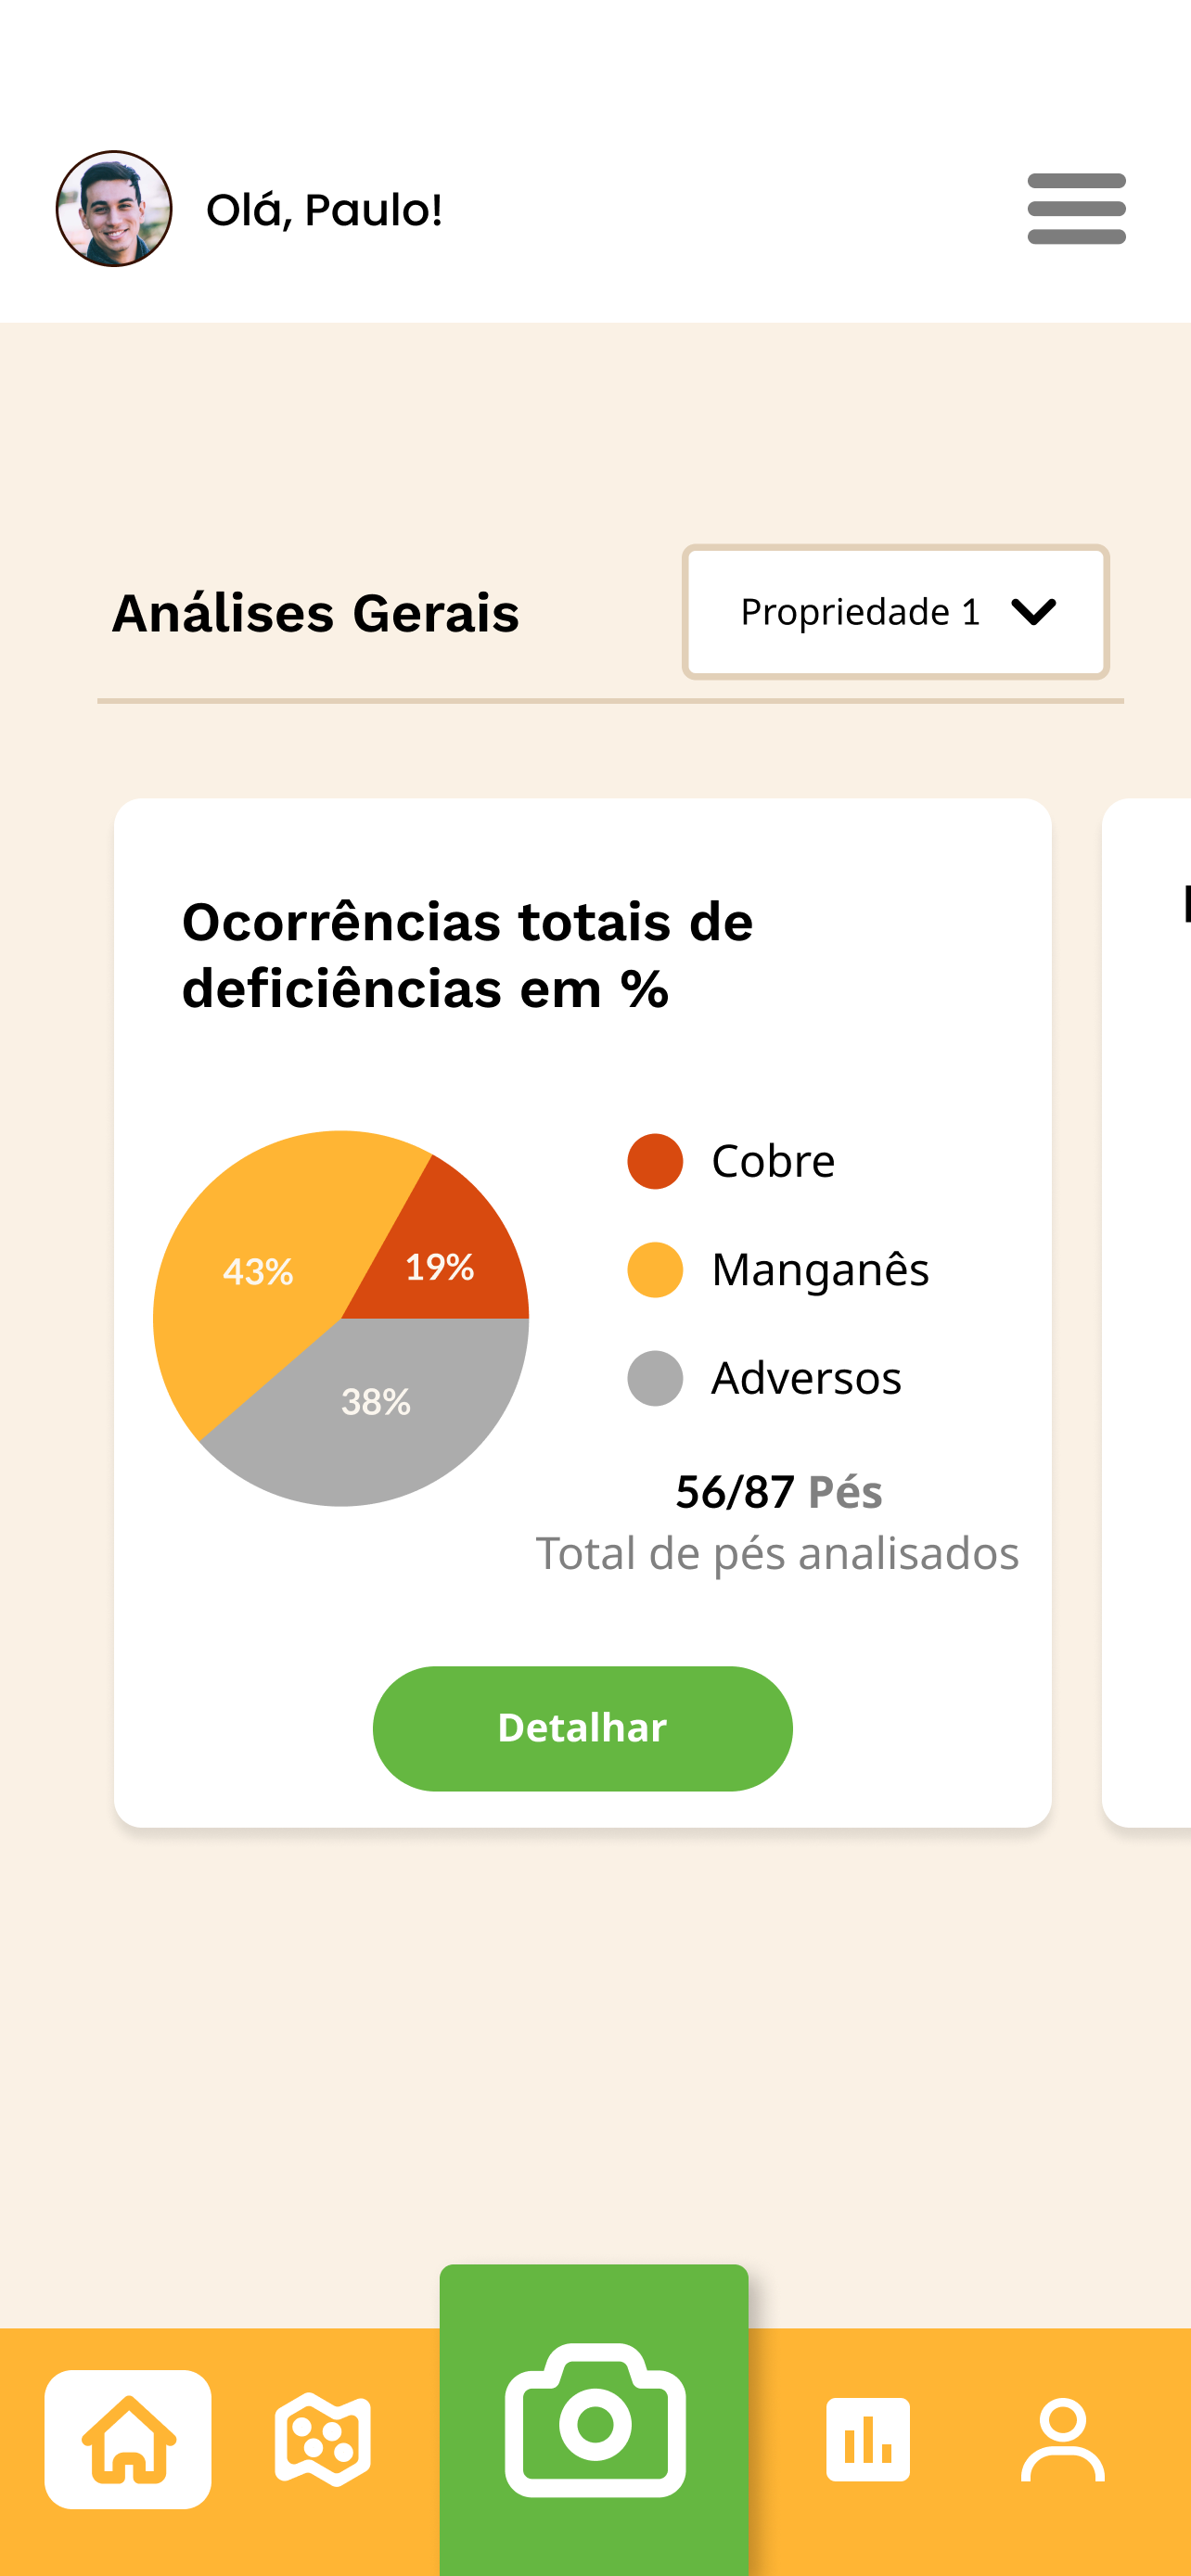
\includegraphics[width=0.2\textwidth]{Images/MobileInicio.png}
\SourceOrNote{Equipe 21 - Vitalliz (2025)}
\end{figure}

O menu inicial mobile apresenta as principais funcionalidades do sistema de forma
otimizada para dispositivos móveis, garantindo fácil acesso e navegação.
\medskip



\begin{figure}[H]
\centering
\caption{Protótipo Interface Web - Tela de Histórico}
\label{fig:interface-web-telahistorico-1}
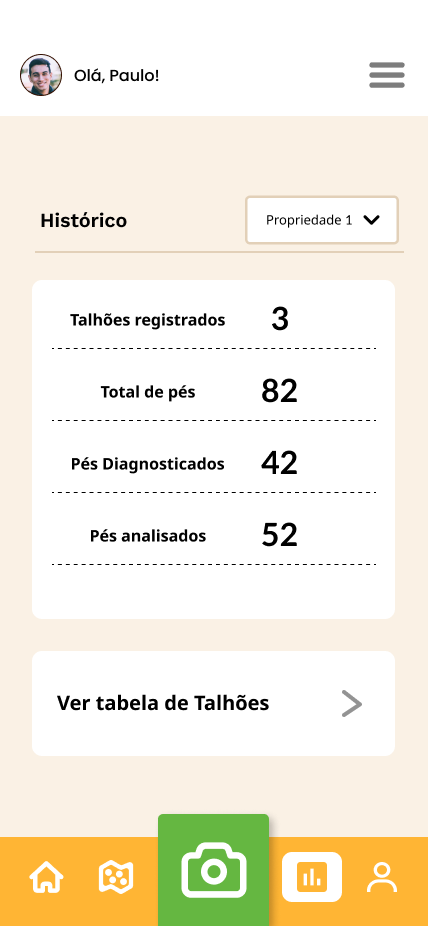
\includegraphics[width=0.2\textwidth]{Images/MobileHistorico.png}
\SourceOrNote{Equipe 21 - Vitalliz (2025)}
\end{figure}

A tela de histórico mobile também apresenta a visão geral das análises e cadastros da 
propriedade, com layout otimizado para telas menores.
\medskip



\begin{figure}[H]
\centering
\caption{Protótipo Interface Mobile - Tela de Resultados}
\label{fig:interface-mobile-tela-resultados}
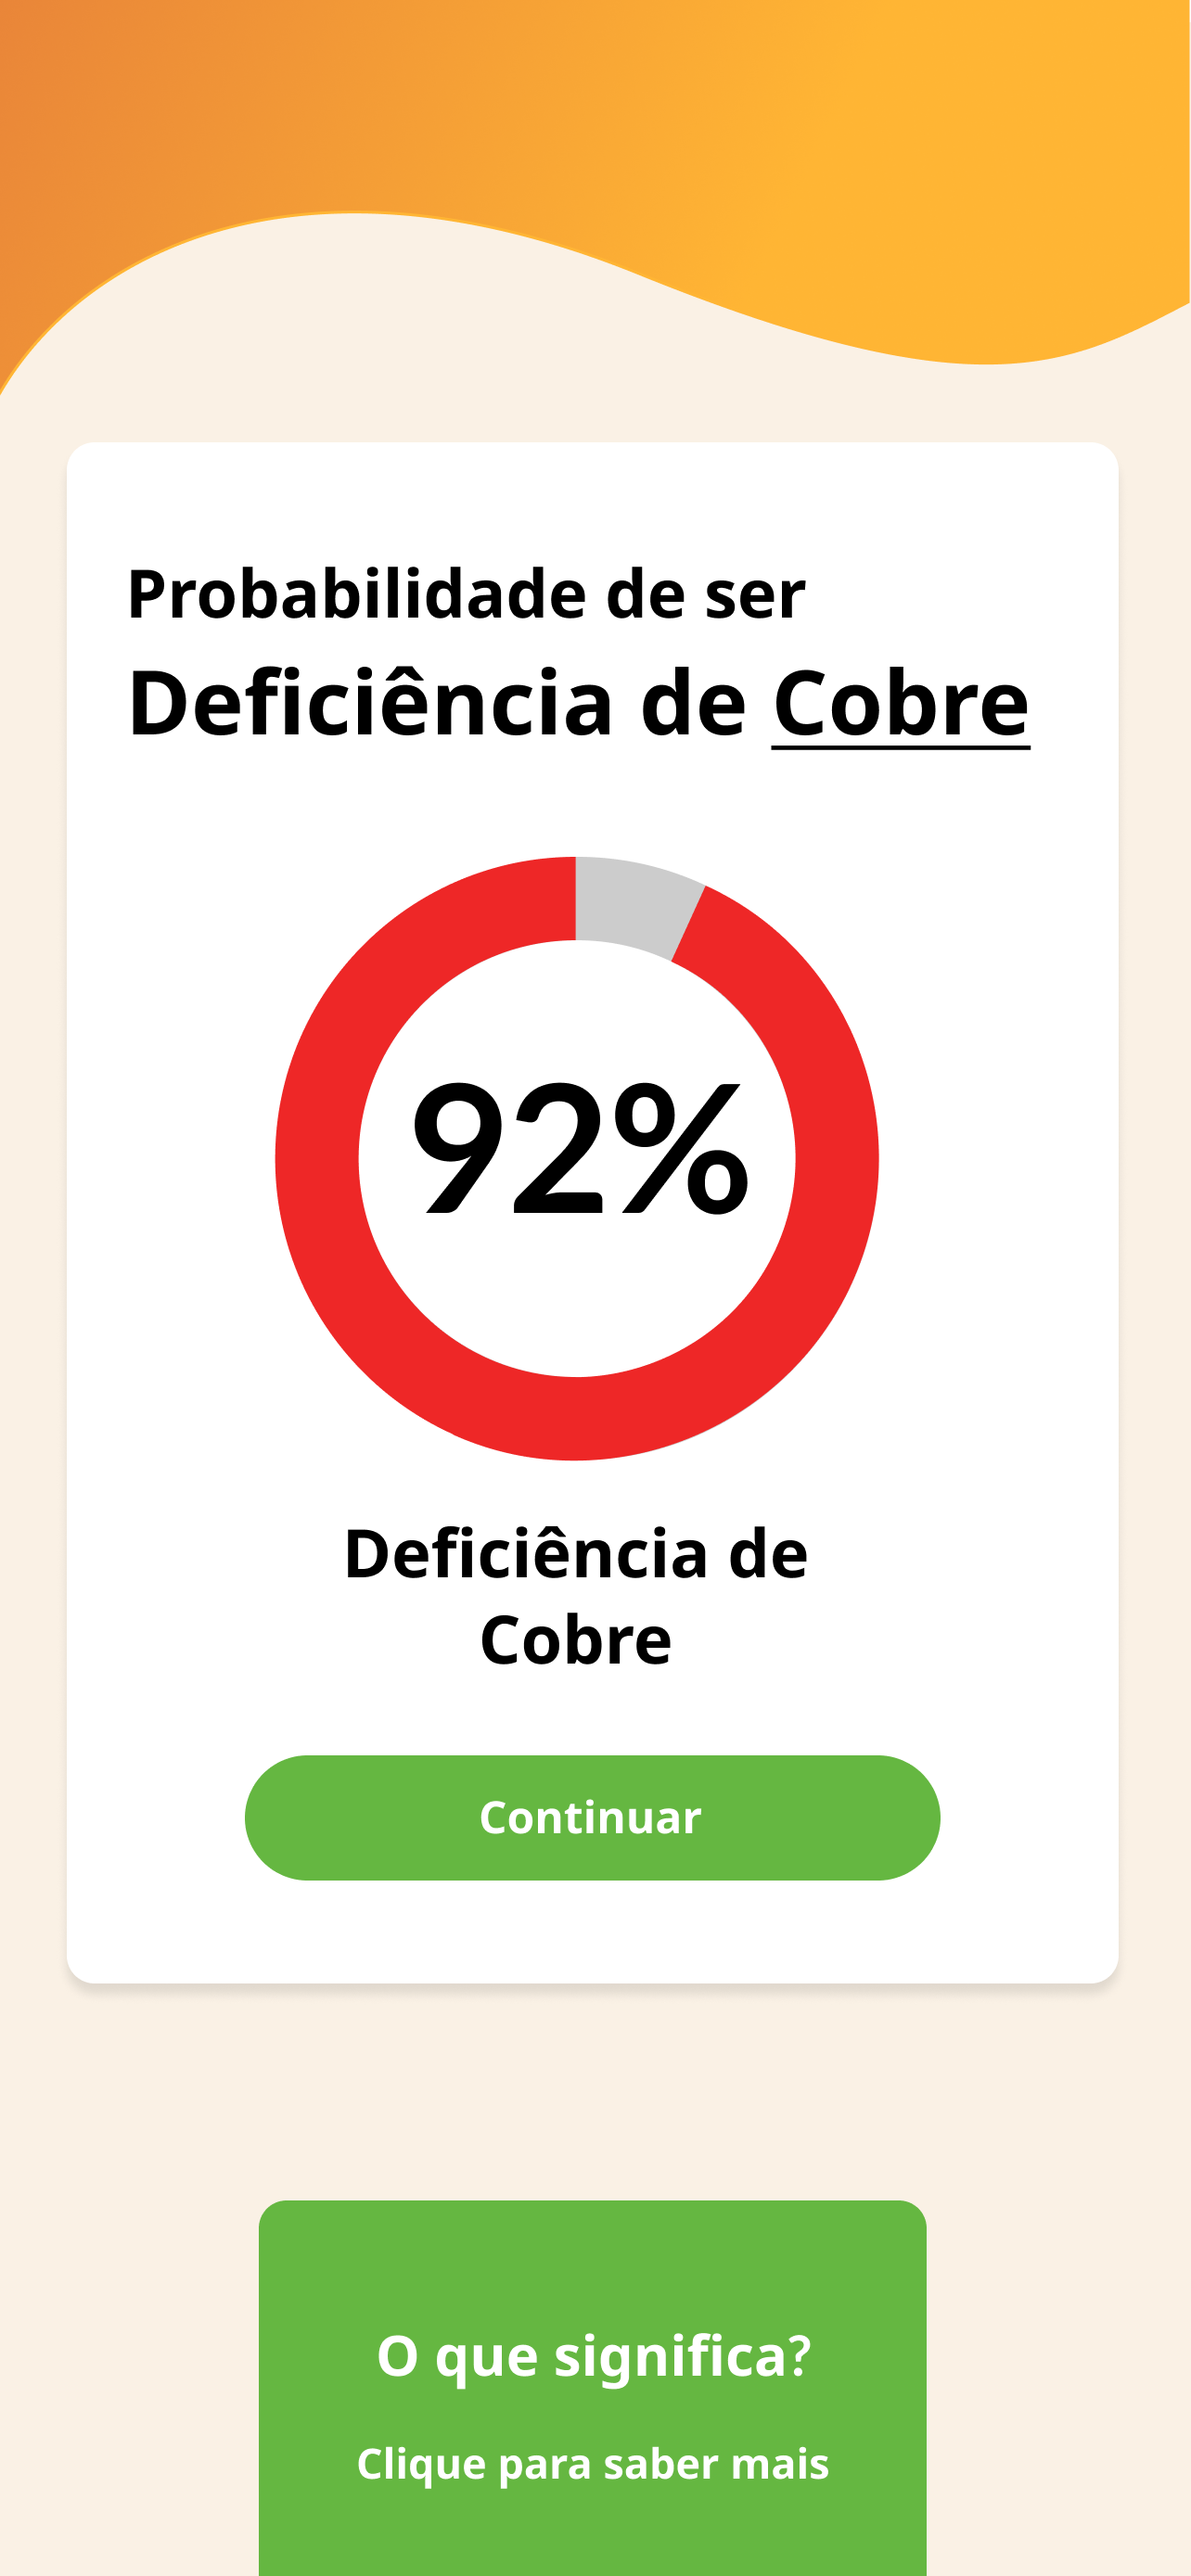
\includegraphics[width=0.2\textwidth]{Images/MobileResultado.png}
\SourceOrNote{Equipe 21 - Vitalliz (2025)}
\end{figure}

A tela de Resultados exibe os resultados detalhados das análises realizadas na
imagem enviada, permitindo melhor visualização do diagnóstico.
\medskip


\begin{figure}[H]
\centering
\caption{Protótipo Interface Mobile - Tela de Mapa}
\label{fig:interface-mobile-tela-mapa}
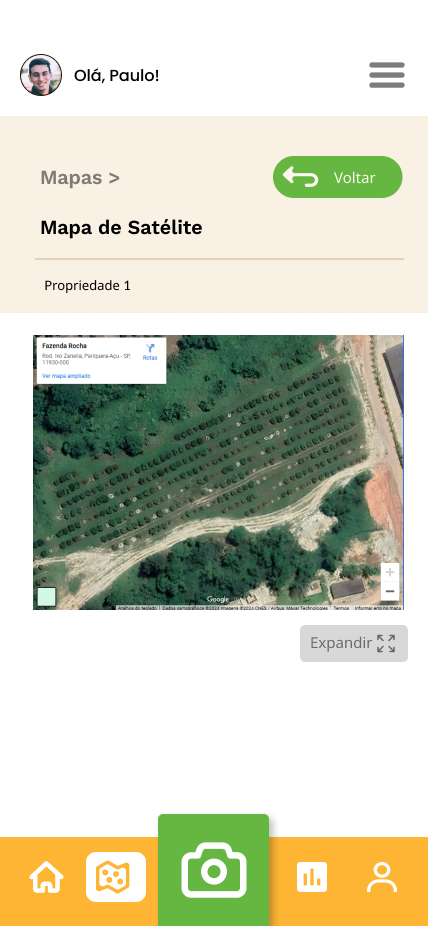
\includegraphics[width=0.2\textwidth]{Images/MobileMapa.png}
\SourceOrNote{Equipe 21 - Vitalliz (2025)}
\end{figure}

Nesta tela, o usuário pode visualizar os talhões de sua propriedade em um
mapa interativo.
\medskip